\section{Introduction}
After training the reinforcement learning agent and tuning its model parameters based on the 2022/23 EPL season, I evaluated it against the complete 2023/24 season. Training was conducted over 30 iterations and the trained agent was evaluated on a similar number of iterations. I used the average points accrued over the season as the key metric used to evaluate the FPL agent. Its performance was contrasted against two other agents:
\begin{itemize}
    \item Baseline agent - average FPL managers' scores per gameweek
    \item Dream Team agent - the 11 highest scoring players from the 2023/24 season in an eligible FPL formation
\end{itemize}
Further, I also report my agent's percentile ranking during the 2023/24 season, had it managed its own team.

\section{Agent Performance Overview}
My agent accumulated an average total of 1083 points across the 2023/24 season. This represented a 1st percentile score among all FPL managers. The agent faired rather poorly against the baseline agent, which scored an average of 1830 points. The dream team agent, too, outperformed my agent, achieving a score of 2217. \cite{fantasyfootballpundit2024}

\section{Gameweek-by-Gameweek Analysis}
Both the training \ref{fig:train_average_gameweek_performance} and the testing data \ref{fig:test_average_gameweek_performance} show distinct variance in sequential gameweek points earned by the agent. The 2023/24 season saw an unprecedented level of injuries across Premier League clubs. Overall injury incidences increased by about 11\% compared to the previous season \cite{analyticsFC2024}. The agent could not take advantage of extra transfers or chips like Freehit and Wildcard, which would have enabled it to transfer out extra injured players.

Furthermore, the agent could not maximize Blank and Double Gameweeks. A Blank Gameweek contains fewer than the normal 10 matches, with at least one club having no fixture, and players from such a club having no chance of scoring Fantasy points. A Double Gameweek contains more than the normal 10 fixtures, with at least one club playing two fixtures in one gameweek, thus players from that club have two chances to core Fantasy points. Blank and Double Gameweeks usually occur due to Premier League teams playing in tournament matches that have conflicting match schedules with the Premier League e.g. the FA Cup or the Champions League. They may also occur due to unforseable circumstances e.g. poor weather, where a game is postponed. Chips like free hit come in handy in such gameweeks where one can replace your entire team to cater for gameweek-specific needs.

\begin{figure}[h]
    \centering
    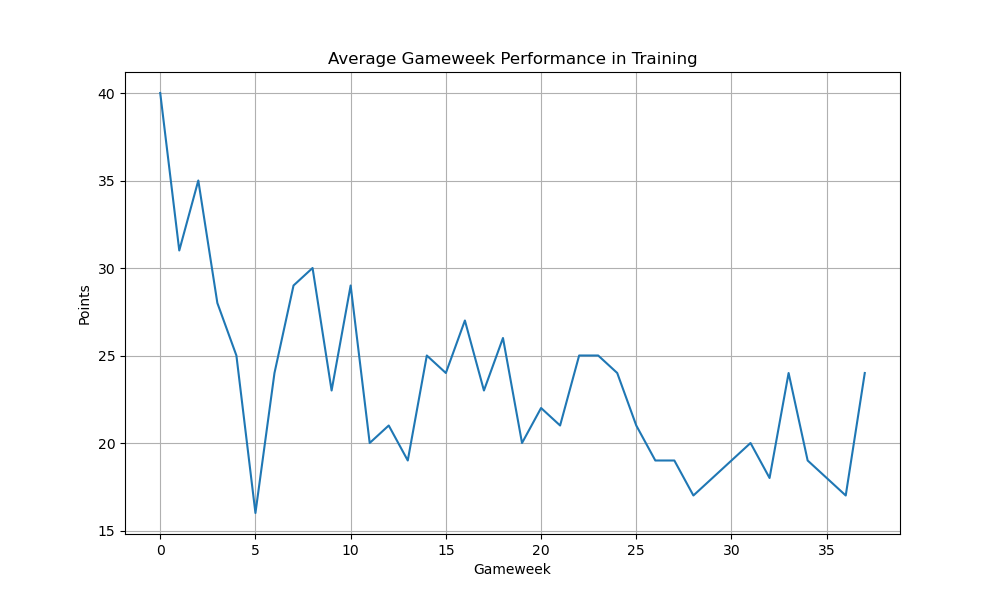
\includegraphics[width=1.0\textwidth]{figs/train_average_gameweek_performance.png}
    \vskip 0.2in
    \caption{Average points per gameweek [training]}
    \label{fig:train_average_gameweek_performance}
\end{figure}

\begin{figure}[h]
    \centering
    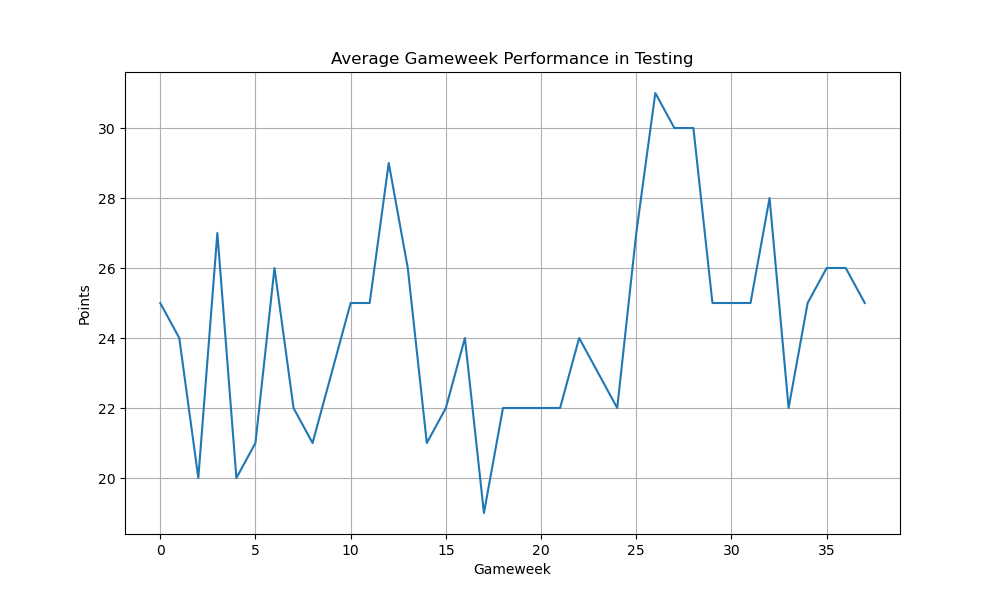
\includegraphics[width=1.0\textwidth]{figs/test_average_gameweek_performance.png}
    \vskip 0.2in
    \caption{Average points per gameweek [testing]}
    \label{fig:test_average_gameweek_performance}
\end{figure}

\section{Algorithm Analysis}
The main parameters that I experimented with while training my agent were the number of actions $a$ and the future reward discount factor $\lambda$. There was no significant change in points while varying the $a$. This likely suggests that my simplified action space with dynamically maintained subsets was effective regardless of size through periodic replacement of the weakest members as discussed in \ref{action_space}. This observation might further suggest that my agent sufficiently explored promising team selections through VPI, reinforcing the approach taken by Matthew et al. \cite{matthews2012}.

However, I found that a discount factor of 0.5 resulted in the highest average points during testing as discussed in \ref{fig:learning_curve_0.5}. A discount factor of 0.9 showed great promise during the initial episodes by quickly dwindled off, while the agent with the 0.5 discount factor closed off strongly after training with about 1130 points. The high discount factor (0.9) placed greater importance on future rewards, leading to an excessive focus on long-term potential at the expense of immediate points. A balanced discount factor (0.5) allowed the agent to give moderate importance to both immediate rewards and future potential. This allowed it to adapt better to the changing dynamics of the 2023/24 season, especially the complex blank and double gameweeks in the latter part of the season.

\begin{figure}[h]
    \centering
    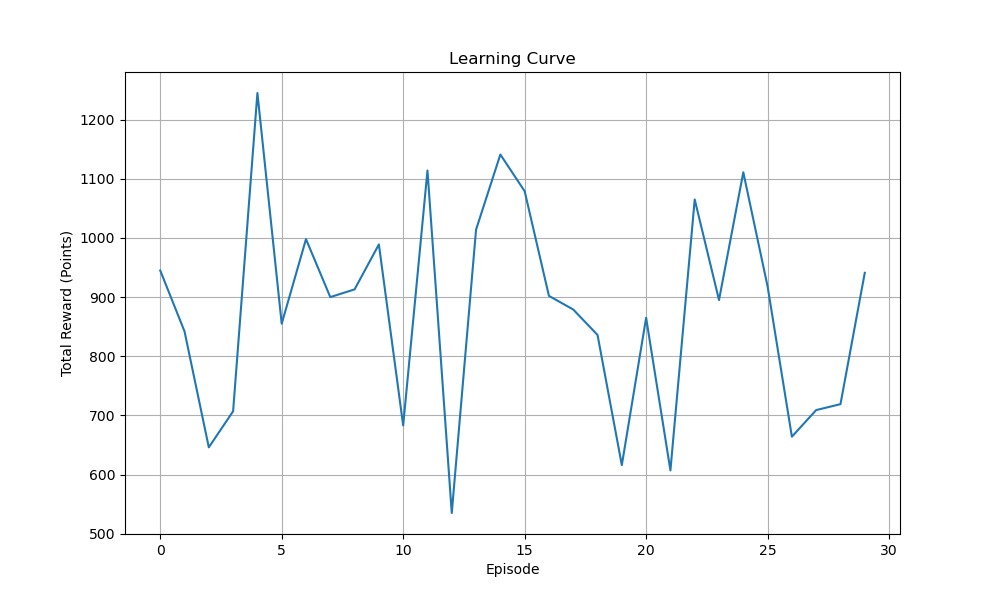
\includegraphics[width=1.0\textwidth]{figs/learning_curve_0.3.png}
    \vskip 0.2in
    \caption{Agent learning curve with a discount factor of 0.3}
    \label{fig:learning_curve_0.3}
\end{figure}

\begin{figure}[h]
    \centering
    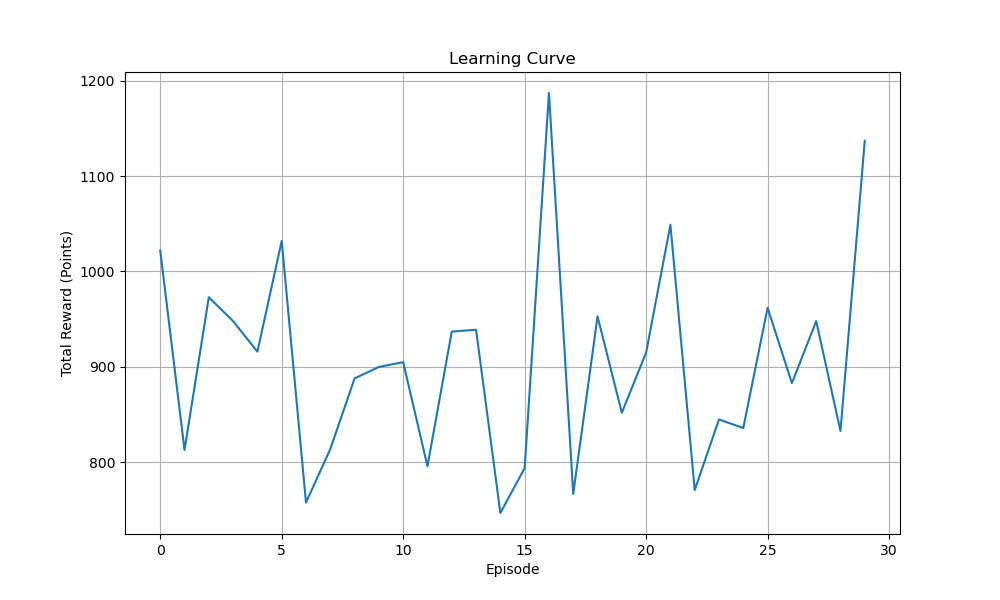
\includegraphics[width=1.0\textwidth]{figs/learning_curve_0.5.png}
    \vskip 0.2in
    \caption{Agent learning curve with a discount factor of 0.5}
    \label{fig:learning_curve_0.5}
\end{figure}

\begin{figure}[h]
    \centering
    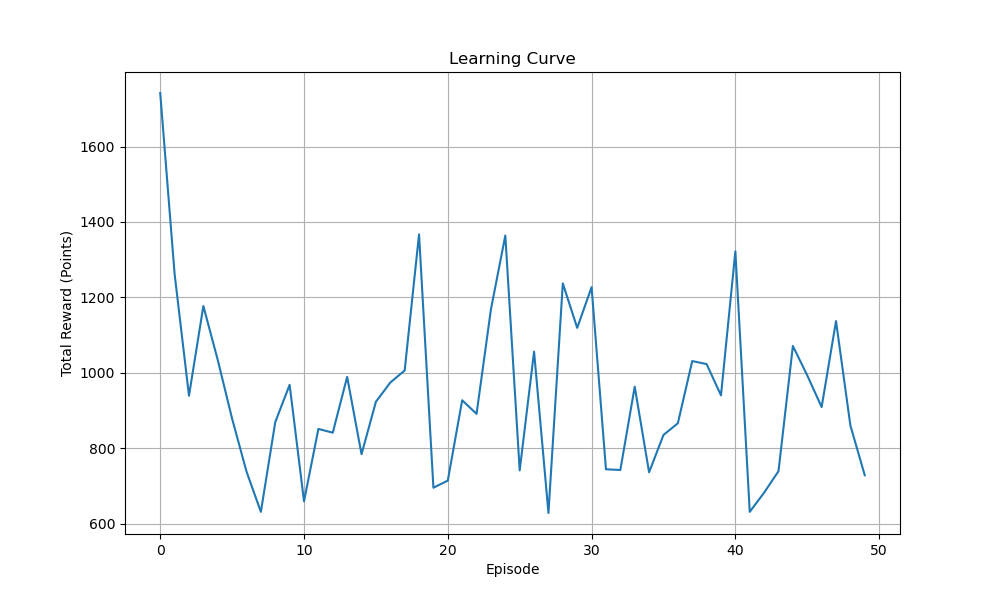
\includegraphics[width=1.0\textwidth]{figs/learning_curve_0.9.png}
    \vskip 0.2in
    \caption{Agent learning curve with a discount factor of 0.9}
    \label{fig:learning_curve_0.9}
\end{figure}
